\documentclass[12pt]{article}

\title{Journal for Complex Analysis}
\author{Michael Gavina}


\usepackage{amssymb,amsfonts,amsmath,amsthm,url,graphicx}
\graphicspath{ {./images/} }


%\pagestyle{empty} % for no page numbers
\setlength{\oddsidemargin}{-.1in}      % 1in left margin
\setlength{\evensidemargin}{-.1in}     % 1in left margin (even pages)
\setlength{\topmargin}{0in}           % 1.50in top margin
\setlength{\textwidth}{6.7in}           % 6.3in text - 1.25in rt margin
\setlength{\textheight}{9in}            % Body ht for 1in margins
\addtolength{\topmargin}{-\headheight}  % No header, so compensate
\addtolength{\topmargin}{-\headsep}     % for header height and separation
%  End of margins and formatting params %
\linespread{1}
\setlength{\parindent}{0pt}


\usepackage{color}
\definecolor{cherry}{rgb}{0.9,.1,.2}
\definecolor{green}{rgb}{.2,.7,0}
\definecolor{blue}{rgb}{0,.0, .81}

\def\green#1{\textcolor{green}{#1}}
\def\cherry#1{\textcolor{cherry}{#1}}
\def\blue#1{\textcolor{blue}{#1}}

\begin{document}
\maketitle

\begin{center}
\textbf{\large Chapter 0}
\end{center}

\noindent{\bf Task 1}
\\
\noindent{\bf a}
$x \mapsto 2x$ \\
Here, the original function is transformed in which only the positive and negative even numbers and zero are shown on the number line. This transformation is similiar to a dialation of a geometric shape.
\\

\noindent{\bf b}
$x \mapsto 2x + 1$ \\
Here, the original function is transformed in which only the the positive and negative odd numbers are shown on the number line. This transformation first dilates then translates the line by one.
\\

\noindent{\bf c}
$x \mapsto -x$ \\
Here, the original function is transformed into the same number line as before. However, the effect the transformation is that of a reflection at zero. This set is an image of the original function. 
\\

\noindent{\bf d}
$x \mapsto -x + 4$ \\
Here, the original function is transformed by a reflection on the line at zero then a translation will be applied to shift the line by four. However, this new set is an image of the original function. 
\\

\noindent{\bf e}
$x \mapsto -3x + 6$ \\
Here, the original function is transformed by a reflection then a translation across the line. Within this new function, the only numbers contained within this set, would be powers of three.
\\

\noindent{\bf Task 2}\\
\noindent{\bf a}
$x \mapsto x^2$ \\
Here, the original function is dilated more as the numbers increase, however, this function only allows positive outputs from the intial values. This means that only half of the number line would be used when the transformation is applied.
\\

\noindent{\bf b}
$x \mapsto x^3$ \\
Here, the original function is similiarly dialated to the last function, however, this time, negative numbers can be a possible output of the function. This allows the full number line to be used when representing the function.
\\

\noindent{\bf c} 
$x \mapsto \frac{1}{x}$ \\
Here, the transformation of this function makes its so that all of the numbers are contained between 0 and 1, and 0 and -1. However, zero is not included within this interval because of its undefined behavior. \\
\noindent{\bf Task 3} \\

\noindent{\bf a} 
$x \mapsto 10^x$ \\
Here, the transformation of the function stretches out the positive side of the line rather extremely while the negative side is non-exsitent. In fact, the line can never cross zero at all, leaving zero as a hole within the line. \\

\noindent{\bf b}
$x \mapsto e^x$ \\
This transformation is similar to the last transformation, however, the factor in which the postive side of the line will stretch will be weaker than the last transformation.\\

\noindent{\bf c} 
$x \mapsto e^{-x}$ \\
This transformation is different from the previous two; the negative numbers will produce postive values which will increase the more negative the number is, while the postive values will only produce values closer and closer to zero, and zero is still a hole.\\

\noindent{\bf d}  
$x \mapsto -e^x$ \\
This transformation will produce the oppisite of the $e^x$ transformation, in which the negative side of the number line will contain numbers while the positve side cannot contain numbers.
This transformation is like a reflection across zero when compared to the $e^x$ transformation. \\

\noindent{\bf e} 
$x \mapsto -e^{-x}$ \\
This transformation is similiar to the last transformation, in which, it too, is like a reflection across zero, when compared to the $-e^x$ function.\\

\noindent{\bf f} 
$x \mapsto \sin(x)$ \\
Here this transformation is different from the other transformation because when the transformation is finished, the domain is restricted to -1 to 1. 
This is because sine is restricted to $-\frac{pi}{2}$ to $\frac{pi}{2}$, any values greater than the domain, the range will be previous values. \\

\noindent{\bf g} 
$x \mapsto \cos(x)$ \\
This transformation is very similiar to the last transformation, however, cosine has a different domain. 
The domain for cosine is $0$ to $pi$, after this, any domain values will produce previous range values.\\

\noindent{\bf Task 4}\\
There are two parts to this question.\\ 

Why are properties (F5) and (F6) not true for $\mathbb{N}$?\\

For F5, given that natural numbers are all of the numbers that are not negative, there is not an addivitive inverse of any of the natural numbers included within the natural numbers set. \\

For F6, given that natural numbers are all positve whole numbers, there is never a number in which $\frac{p}{q}$ can ever be true. Thus, there is never a multiplicative inverse.\\


\noindent{\bf Task 5}\\
There are two parts to this question.\\

Which properties are true for each set of sets: $\mathbb{Z}$, $\mathbb{Q}$?\\

For $\mathbb{Z}$, every property will apply except for F6, in which, there is never such a case in which a fractional number can be apart of this set. 
Since the numbers are all integers, the basic rules apply for all intergers (F1-F3), Here $0$ and $1$ are included within this set (F4), and negative numbers exist within this set (F5).\\

For $\mathbb{Q}$, every property will apply for this set. 
Since the numbers are fractional, they can be added and multiplied. 
This also allows for the communtaive and associative property to be true as well and thus (F1-F3) are true.
$0$ and $1$ are included within this set and thus (F4) is true. 
Negative fractions and positive fractions of the same value can exist within this set and thus (F5) is true.
Inverse fractions of fractional and whole numbers do exist within this set and thus (F6) is true.\\

\noindent{\bf Task 6}\\

The rules of ordered sets are that of which there are numbers within the set that are bigger and that adding two numbers will create a bigger number than $0$ within the set.
Here, it is possible to have fractional elements that will exceptionally small numbers but nonetheless still be bigger than $0$. 
The only way in which $0$ could be a possible would to have $0$ as one of the possible numbers as $a$ or $b$, which breaks the ruling for order sets.
Thus, $\mathbb{Q}$ is an ordered set.\\

\noindent{\bf Task 7}\\

Within A, the number $\frac{1}{2}$ resides, while within B, the number $2$ is within the set.\\

Within both sets, there are restrictions on the value of both $q$ and $p$. 
Solving the inequality shows that for set A, the fractional representation that is outputed from the set must follow this ruling: $\frac{p^2}{q^2} < 2$.
Similiarly, there a inequality that must be followed for set B: $\frac{p^2}{q^2} > 2$. 
Here it is clearly shown that set B will contain bigger numbers always, because it's fractional representation must always be bigger than 2.\\

However, both of these sets are not Dedekind complete because of the rulings. 
Both sets can never contain the irrational number $\sqrt(2)$. 
Thus, in both sets, there is a hole located at $\sqrt(2)$.\\

\noindent{\bf Task 8}\\

For $\mathbb{N}$, this is representation of the number line only containing, positive whole numbers aswell as $0$.\\

For $\mathbb{Z}$, this is representation of all of the positive and negative whole numbers along with $0$.\\

For $\mathbb{Q}$, this is representation of all of the numbers across the number line that are not irrational.\\

\noindent{\bf Task 9}\\

\begin{center}
	\begin{tabular}{| c c c |}
	\hline
		Task 1 & ]0,1[ & [2,5]\\
	\hline\hline
		A. & ]0,2[ & [4,10]\\
	\hline
		B. & ]0,3[ & [5,11]\\
	\hline 
		C. & ]-1,0[ & [-5,-2]\\
	\hline
		D. & ]3,4[ & [1,2]\\
	\hline
		E. & ]3,6[ & [-11,0]\\
	\hline
	\end{tabular}
\end{center}


\begin{center}
	\begin{tabular}{| c c c |}
	\hline
		Task 2 & ]0,1[ & [2,5]\\
	\hline\hline
		A. & ]0,1[ & [4,25]\\
	\hline
		B. & ]0,1[ & [8,125]\\
	\hline 
		C. & ]0,1[ & [$\frac{1}{5}$,$\frac{1}{2}$]\\
	\hline
	\end{tabular}
\end{center}


\begin{center}
	\begin{tabular}{| c c c |}
	\hline
		Task 3 & ]0,1[ & [2,5]\\
	\hline\hline
		A. & ]0,10[ & [100,100000]\\
	\hline
		B. & ]1,$e$[ & [$e^2$, $e^5$]\\
	\hline 
		C. & ]0,$\frac{1}{e}$[ & [$\frac{1}{e^5}$, $\frac{1}{e^2}$]\\
	\hline
		D. & ]$-e$, 1[ & [$-e^5$, $-e^2$]\\
	\hline
		E. & ]$-\frac{1}{e}$,0[ & [$-\frac{1}{e^2}$,$-\frac{1}{e^5}$]\\
	\hline
		F. & ]0,$sin(1)$[ & [$-1$, $sin(2)$]\\
	\hline
		G. & ]$cos(1)$,1[ & [$-1$, $cos(5)$]\\
	\hline
	\end{tabular}
\end{center}

\begin{center}
\textbf{\large Chapter 1}
\end{center}


\noindent{\bf Task 10} Find four complex numbers such that when placed on an Argand diagram, they are located at the vertices of a square.\\

%insert the image here
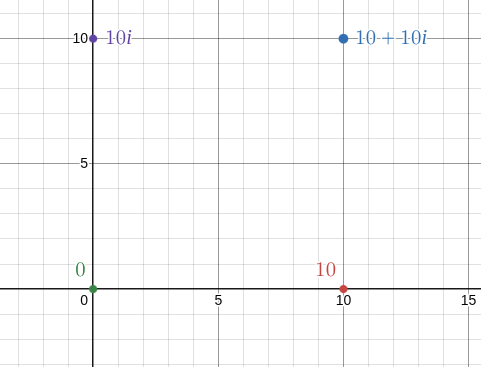
\includegraphics[scale=.5]{./images/task10.png}

Here the points I picked were:\\
$10, 10+10i, 10i, 0$.\\



\noindent{\bf Task 11} Show that the expression for $z + w$ and $z * w$ in the previous definition match the results you get by treating each complex number as a binomial and adding or multiplying them according to the rules of polynomials, replacing $i^{2}$ with $-1$ wherever it appears.\\


There are two parts to this question: $z*w$ and $z+w$\\

$z = x + yi$ and $w = u + vi$\\

Starting with $z*w$:\\
$z * w = (x + yi) * (u + vi)$\\
$z * w = x*u + u*yi + x*vi + y*v*i^2$\\
$z * w = x*u + u*yi + x*vi - y*v$\\
$z * w = (x*u - y*v) + (u*y + x*v)i$\\

Next $z+w$:\\
$z + w = (x+yi) + (u + vi)$\\
$z + w = x + u + yi + vi$\\
$z + w = (x + u) + (y + v)i$\\

\noindent{\bf Task 12} For each pair of complex numbers $z$ and $w$ given below, compute $z + w$ and $zw$.
Then plot all four numbers $z,w, z + w$ and $zw$ on an Argand diagram.\\

% insert images
 
\noindent{\bf a}
$z = 4, w = i$\\
$z + w = 4 + i$ and $z*w = 4i$\\
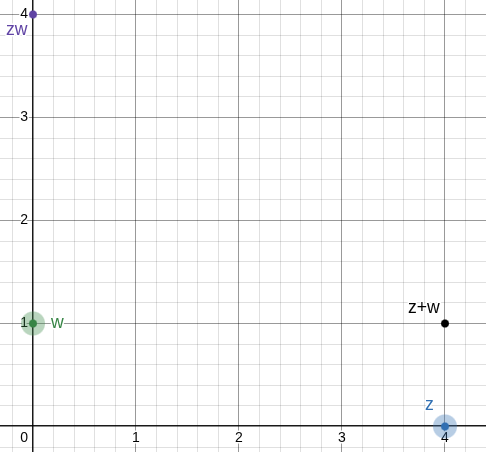
\includegraphics[scale=0.25]{./images/task12a.png}\\

\noindent{\bf b}
$z = 3 + 5i, w = -i$\\
$z + w = 3 + 4i$ and $z*w = -5 - 3i$\\
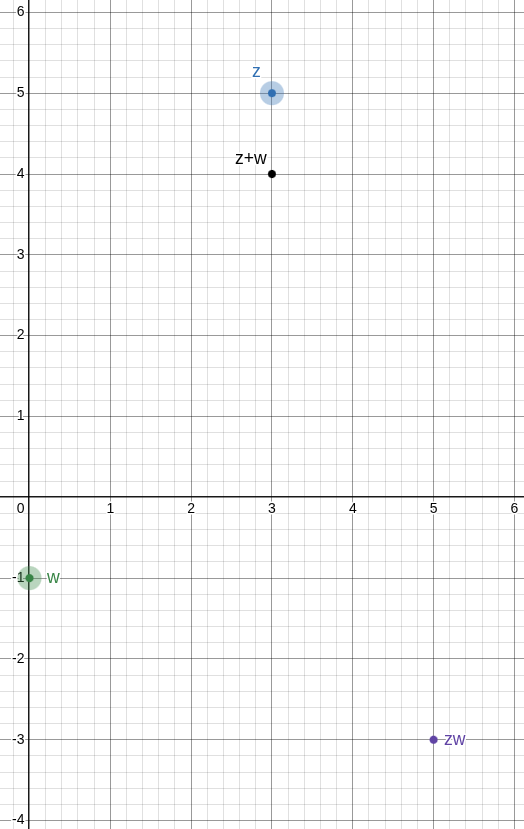
\includegraphics[scale=0.25]{./images/task12b.png}\\


\noindent{\bf c}
$z = 1 + i, w = -1 - i$\\
$z + w = 0$ and $z*w = -2i$\\
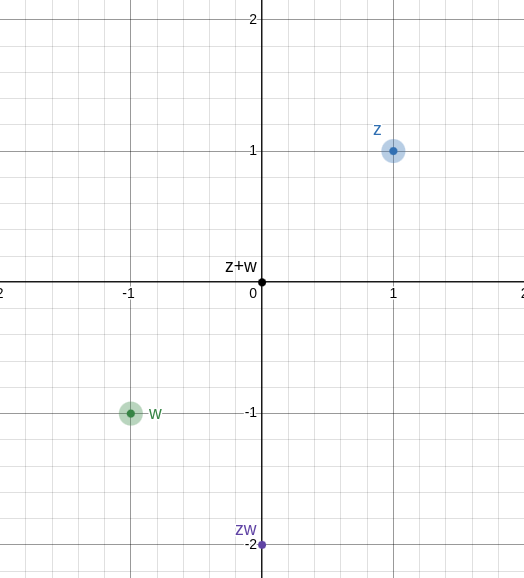
\includegraphics[scale=0.25]{./images/task12c.png}\\

\noindent{\bf d}
$z = -1 + i\sqrt(3), w = -1 - i\sqrt(3)$\\
$z + w = -2$ and $z*w = 4$\\
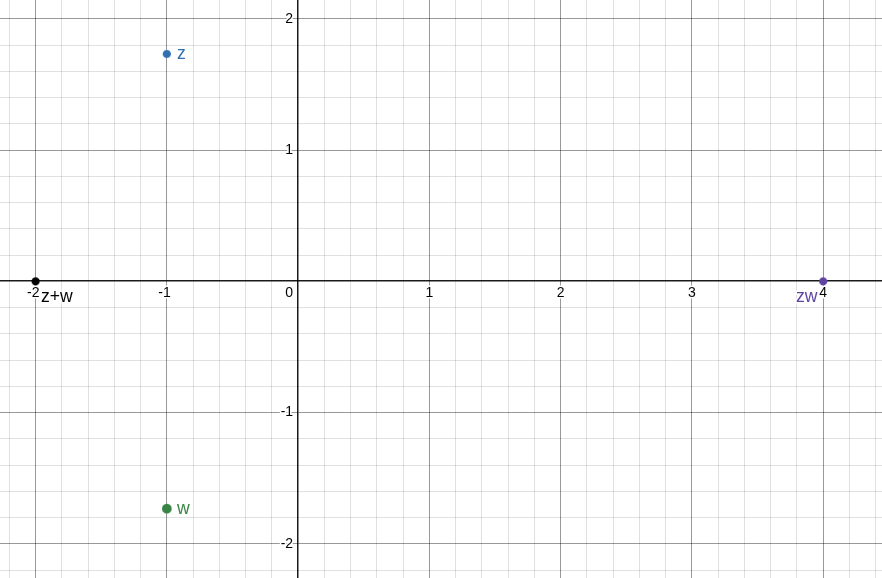
\includegraphics[scale=0.25]{./images/task12d.png}\\


\noindent{\bf e}
$z = 2 + i, w = 3 + i$\\
$z + w = 5 + 2i$ and $z*w = 5 + 5i$\\
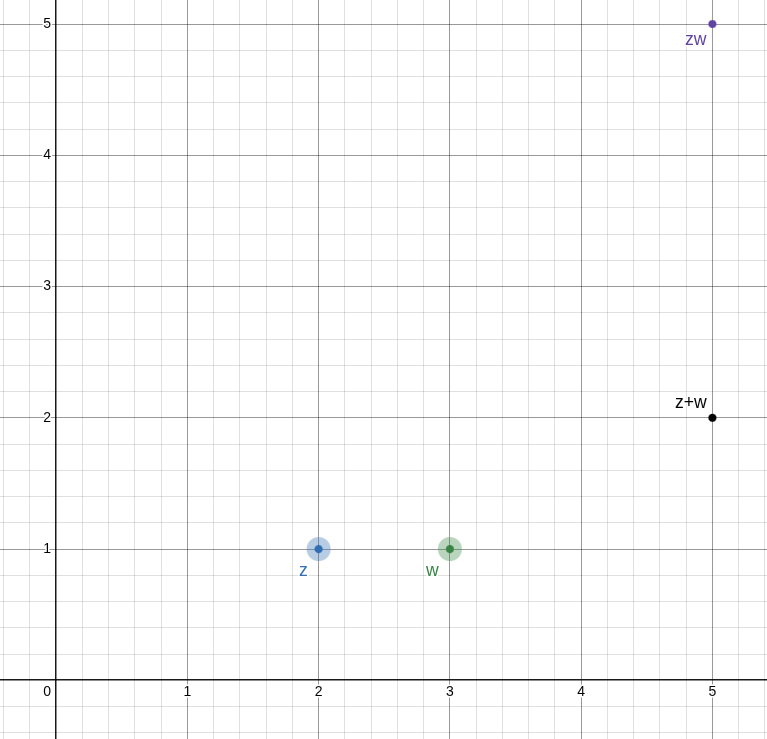
\includegraphics[scale=0.25]{./images/task12e.png}\\


\noindent{\bf Task 13} Suppose $z,w \in \mathbb{C}$. Show that $z + w = w + z$ and $z * w = w * z$.\\

There are two proofs within this question: $z + w = w + z$ and $z * w = w * z$.\\
$w = a + bi$\\
$z = c + di$\\

$z + w = w + z$\\
$a + bi + c + di = c + di + a + bi$.\\
Since there is only real numbers contained within $a,b,c,d$, the rules of addition will apply.\\


$z * w = w * z$\\
$(a + bi)(c + di) = (a*c + a*di + c*bi - b*d)$\\
Since there is only real numbers contained within $a,b,c,d$, the rules of mulitplication will apply.\\


\noindent{\bf Task 14} Suppose that $z_1,z_2,w \in \mathbb{C}$. Show that $w(z_1+z_2) = wz_1 + wz_2$.\\

$w = a + bi$\\
$z_1 = c + di$\\
$z_2 = e + fi$\\

$w*(z_1 + z_2) = (a + bi)(c + di + e + fi)$\\
$w*(z_1 + z_2) = a*c + a*e + a*di + a*fi + c*bi - b*d + e*bi - b*f$\\
$w*(z_1 + z_2) = (a*c - b*d + c*bi + a*di) + (a*e - b*f + e*bi + a*fi)$\\
$w*z_1 + w*z_2 = (a+bi)(c+di) + (a+bi)(e+fi)$\\
$w*z_1 + w*z_2 = (a*c + a*di + c*bi - b*d) + (a*e + a*fi + e*bi - b*f)$\\

$w*z_1 + w*z_2 = (a*c + a*di + c*bi - b*d) + (a*e + a*fi + e*bi - b*f) = w*(z_1 + z_2)$\\

Thus, $w*z_1 + w*z_2 = w*(z_1 + z_2)$.\\

\noindent{\bf Task 15}\\
$(1+i)^2 = 2i$\\
$(1+i)^3 = -2 + 2i$\\
$(1+i)^4 = -4$\\

When ploting the points on a graph, the graph produced a spiral type shape that was counter clockwise.\\
%insert image
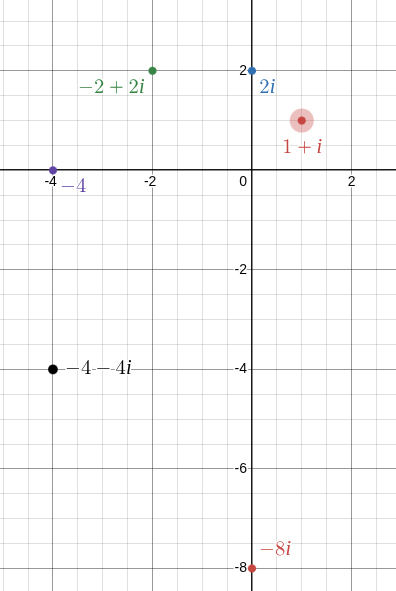
\includegraphics[scale=0.25]{./images/task15a.png}


The same happened when ploting the $(1-i\sqrt{3})$, the only difference was the spiral that was produced went clockwise instead of counter clockwise.\\
%insert image
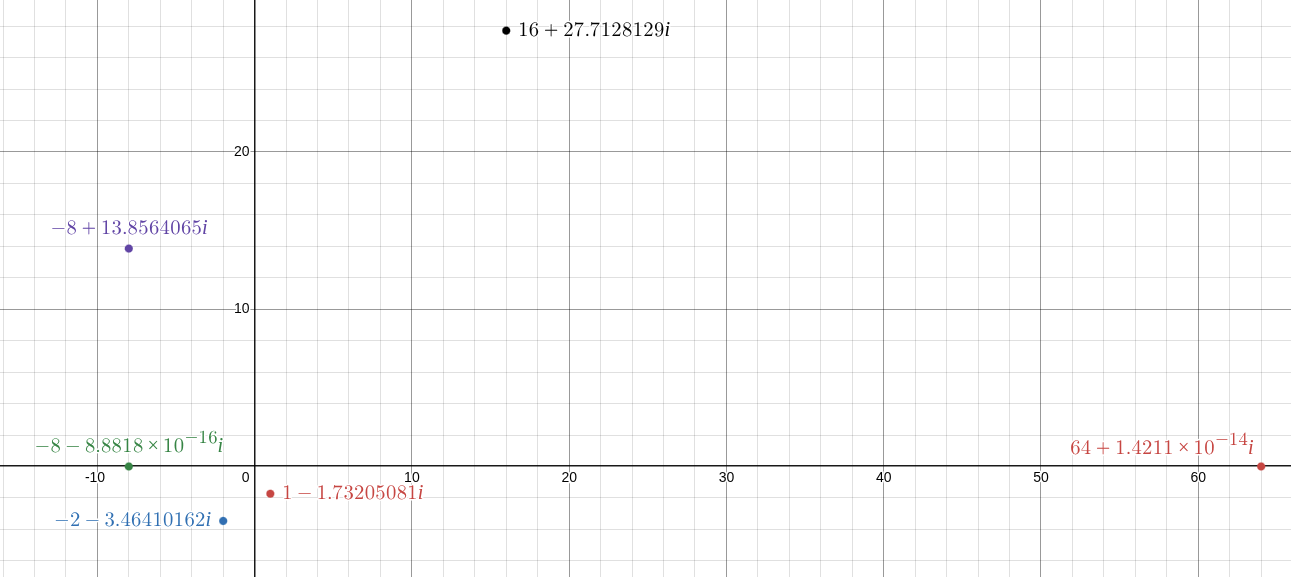
\includegraphics[scale=0.25]{./images/task15b.png}


\noindent{\bf Task 16}\\
The basic pattern I noticed was that for the first four powers of $\i$, they were unique values. 
However, after that, the values tend to repeat in a perdictable pattern.\\ 

$i^{99} = -i$\\
$i^{1001} = i$\\
$i^{57368} = 1$\\

\noindent{\bf Task 17}\\

$z * z^{-1} = (x + y\i)(\frac{x}{x^2+y^2} - \frac{y}{x^2+y^2}i)$\\
$z * z^{-1} = \frac{x^2}{x^2+y^2} - \frac{x*yi}{x^2+y^2} + \frac{x*yi}{x^2+y^2} + \frac{y^2}{x^2+y^2}$\\
$z * z^{-1} = \frac{x^2+y^2}{x^2+y^2}$\\
$z * z^{-1} = 1$\\

\noindent{\bf Task 18}\\

$i^{-1} = -i$\\

$(3+4i)^{-1} = \frac{3}{25} - \frac{16}{25}i$\\

$(\frac{1}{2} - \frac{1}{2}i)^{-1} = 1 + 1i$\\

$(-\frac{1}{2} + \frac{\sqrt{3}}{2}i)^{-1} = (-\frac{1}{2}-\frac{\sqrt{3}}{2})$\\


\noindent{\bf Task 19}\\
Task 11, 13, 14, and 17 all prove rules F1, F2, F3, and F6.
As well as a 1 and a 0 being included within this set, that proves F4. 
We also know that a or b must be a real number, which has a additive inverse, which proves F5.\\

Thus, $\mathbb{C}$ is a field.

\noindent{\bf Task 20}\\

\noindent{\bf a}\\
$4z = -8i$\\
$z = -2i$\\

\noindent{\bf b}\\
$4iz = -8i$\\
$z = -2$\\

\noindent{\bf c}\\
$4iz = -8$\\
$z = -2i\exp(-1) = 2i$\\


\noindent{\bf d}\\
$z(1-i) = 4$\\
$z = \frac{4}{1-i}$\\


\noindent{\bf e}\\
$z^2 = -4$\\
$z = 2i$\\


\noindent{\bf Task 21}\\

Lets assume that the real component of the $z$ is used to measure the relation between two different $z$ objects. 
Then it would follow that the bigger the real value on one object would mean that the object comes after the one with the smaller real value.\\

However, OF2 would break this continunity. 

Given an object with a large imaginary conponent and an even real number, when multiplied with another imaginary number, the result would be a negative number which would break OF2. 

Thus, $\mathbb{C}$ is not an ordered field.

\noindent{\bf Task 22}\\

\noindent{\bf a}\\
$5 - 3i$\\

\noindent{\bf b}\\
$-5 + 3i$\\

\noindent{\bf c}\\
$3i(1-2i) = 6+3i$\\

\noindent{\bf d}\\
$-3i(1+2i) = 6-3i$\\

\noindent{\bf e}\\
$-i^{99} = -i^3 = i$\\

\noindent{\bf Task 23}\\

$z = x + yi$\\
$\bar{z} = x - yi$\\
$w = a + bi$\\
$\bar{w} = a - bi$\\


\noindent{\bf a}\\

$\overline{x-yi} = x + yi$\\
Here the conjugate of the conjugate is the original object.\\

\noindent{\bf b}\\
$x-yi+a-bi = \overline{x+yi} + \overline{a+bi}$\\
Here the addition of the cojugates is the same as taking the conjugates of the objects individually.\\

\noindent{\bf c}\\
$w*z = a*x + a*yi + x*bi - y*b$ \\


$\overline{w*z} = a*x - y*b - a*yi - x*bi$\\

$\bar{w} * \bar{z} = (x-yi)(a-bi)$\\
$\bar{w} * \bar{z} = a*x - x*bi - a*yi - y*b$\\
$\bar{w} * \bar{z} = a*x - x*bi - a*yi - y*b = \overline{w*z}$\\

Here, both sides of the equation produce the same result when expanded.\\


\noindent{\bf d}\\
$z + \bar{z} = x + yi + x - yi$\\
$z + \bar{z} = 2x$\\
$2\Re(z) = 2(x)$\\

$2\Re(z) = 2x = z + \bar{z}$.

Here, both sides of the equation produce the same result when expanded.\\

\noindent{\bf e}\\

$z - \bar{z} = x + yi - (x - yi)$\\
$z - \bar{z} = yi + yi$\\
$z - \bar{z} = 2yi$\\

$ 2i\Im(z) = 2i(y)$\\

$ 2i\Im(z) = 2iy = z - \bar{z}$\\

Here, both sides of the equation produce the same result when expanded.\\

\noindent{\bf f}\\

$z^{-1} = \frac{x}{x^2+y^2} - \frac{y}{x^2+y^2}i$\\

$\overline{z^{-1}} = \frac{x}{x^2+y^2} + \frac{y}{x^2+y^2}i$\\
$\overline{z}^{-1} = \frac{x}{x^2 + (-y)^2} - \frac{-y}{x^2 + (-y)^2}$\\

$\overline{z}^{-1} = \frac{x}{x^2 + (-y)^2} + \frac{y}{x^2 + (-y)^2} = \overline{z^{-1}}$\\


Here, both sides of the equation produce the same result when expanded.\\

\noindent{\bf Task 24}\\

Describe the geometric shape defined by the given equations.\\

$z = x + yi$\\
$\bar{z} = x - yi$\\

Within a standard graph, we represent the x and the y as coordinates, we can do the same with the complex, where x equals x and yi equals y in the 2D graph space.\\

{\bf a}\\

$x + yi = x - yi$\\
$x = x$\\

This functionally represents a 1D line, where only x values live.\\

{\bf b}\\

$x + yi = i(x - yi)$\\
$x + yi = y + xi$\\

Here, the varibles equal one another, similiar to $y = x$ in the 2D graph space.\\

{\bf c}\\

$x + yi + x - yi = 1$\\
$2x = 1$\\
$x = \frac{1}{2}$\\

There is only one point and that is $\frac{1}{2}$

{\bf d}\\

$(x + yi)^2 + (x - yi)^2 = 2$\\
$x^2 + 2x*yi + y^2 + x^2 - 2x*yi + y^2 = 2$\\
$x^2 + y^2 + x^2 + y^2 = 2$\\
$2*x^2 + 2*y^2  = 2$\\

This is a standard unit circle.\\

{\bf e}\\

$(x+yi)^{-1} = x - yi$\\
$1 = (x - yi) * (x+yi)$\\
$1 = x^2 - y^2 $\\

This is a hyperbolic function on the plane.\\

\noindent{\bf Task 25}\\

$z = x + yi$\\
$\bar{z} = x - yi$\\


$z*\bar{z} = (x + yi)(x - yi)$\\
$z*\bar{z} = x^2 - x*yi + x*yi - y^2i^2$\\
$z*\bar{z} = x^2 + y^2$\\

In this case, $\sqrt{z*\bar{z}}$ would be the distance from the origin, giving the total length of the vector.\\


\noindent{\bf Task 26}\\

\noindent{\bf a}\\
$|z| = \sqrt{i*-i}$\\
$|z| = 1$\\

\noindent{\bf b}\\
$|z| = \sqrt{1^2 - i^2}$\\
$|z| = \sqrt{2}$\\


\noindent{\bf c}\\
$|z| = \sqrt{(-3)^2}$\\
$|z| = 3$\\

\noindent{\bf d}\\
$|z| = \sqrt{9 + 3}$\\
$|z| = \sqrt{12}$\\

\noindent{\bf e}\\
$|z| = \sqrt{25 + 144}$\\
$|z| = \sqrt{169}$\\
$|z| = 13$\\

\noindent{\bf Task 27}\\

$z = x + yi$\\
$\bar{z} = x - yi$\\
$|z| = \sqrt{x^2 + y^2}$\\

$z^{-1} = \frac{\bar{z}}{|z|}^2$\\

$\frac{x}{x^2+y^2} - \frac{y}{x^2+y^2}i = \frac{x-yi}{x^2 + y^2}$\\
$\frac{x-yi}{x^2 + y^2} = \frac{x-yi}{x^2 + y^2}$\\

\noindent{\bf Task 28}\\

$z = x + yi$\\
$|z| = \sqrt{x^2 + y^2}$\\
$w = a + bi$\\
$|w| = \sqrt{a^2 + b^2}$\\


\noindent{\bf a} $|Re z| \leq |z|$\\

$x \leq \sqrt{x^2 + y^2}$\\
This always going to be true.\\


\noindent{\bf b} $|Im z| \leq |z|$\\
$y \leq \sqrt{x^2 + y^2}$\\
Similiar to the last problem, this is always going to be true.\\


\noindent{\bf c} $Re(z\bar{w}) \leq |z||w|$\\
$(x*a) \leq \sqrt{(x)^2 + (y)^2}*\sqrt{(a)^2 + (b)^2}$
Similiar to the last problem, this is always going to be true.\\


\noindent{\bf d} $|z + w| \leq |z|+|w|$\\
$|x + yi + a + bi| \leq (x^2 + y^2) + (a^2 + b^2)$\\
$\sqrt{(x+a)^2 + (y+b)^2} \leq \sqrt{(x^2 + y^2)} + \sqrt{(a^2 + b^2)}$\\
Similiar to the last problem, this is always going to be true.\\

\noindent{\bf Task 29} Prove the triangle inequality: if $a,b,c \in \mathbb{C}$\\
$|a - c| \leq |a - b| + |b - c|$\\
$|a + (b - b) - c| \leq |a - b| + |b - c|$\\
$|a - b + b - c| \leq |a - b| + |b - c|$\\
Here we see that the inequality must be true because we can add $b$ within.\\


\noindent{\bf Task 30} Show that if $z_1,z_2,...,z_n$ is any finite collection of complex numbers, then\\
$|z_1 + z_2 + ... + z_n| \leq |z_1| + |z_2| + ... + |z_n|$.\\

$z_n = a_n + ib_n$\\

Starting with two different $z$ values first we get, 
$\sqrt{(a_1 + a_2)^2 + (b_1 + b_2)^2} \leq \sqrt{a_1^2 + b_1^2} + \sqrt{a_2^2 + b_2^2}$.\\

Let, $z_1 = 2 + 2i$ and $z_2 = 2 - 4i$.\\

Substituting the values in we get, $\sqrt{(2 + 2)^2 + (2 - 4)^2} \le \sqrt{2^2 + (2)^2} + \sqrt{2^2 + (-4)^2}$.\\
$\sqrt{16 + 4} \le \sqrt{8} + \sqrt{20}$.\\
Here it is shown that the inequality has held for this example.\\



Here, we know that this must hold because when we add to imaginary vectors, they could point in different directions of each other. 
This would cause the shortest distance between 0 and the combined vectors to be shorter than the combined vectors.\\

Adding more vectors would only change the shortest path of the combine vectors.\\

Thus, the inequality must hold for a finite collection of complex numbers.\\


\noindent{\bf Task 31}\\
$z = x + yi$\\
$|z| = \sqrt{x^2 + y^2}$\\
$w = a + bi$\\
$|w| = \sqrt{a^2 + b^2}$\\

$|z * w| = |x*a + a*yi + x*bi - y*b|$\\
$|z * w| = \sqrt{x^2*a^2 + y^2*b^2 + a^2*y^2 + x^2*b^2}$\\

$|z| * |w| = |x + yi| * |a + bi|$\\
$|z| * |w| = \sqrt{x^2 + y^2} * \sqrt{a^2 + b^2}$\\
$|z| * |w| = \sqrt{x^2 + y^2} * \sqrt{a^2 + b^2}$\\
$|z| * |w| = \sqrt{a^2*x^2 + b^2*y^2 + y^2*a^2 + x^2*b^2}$\\
$|z| * |w| = \sqrt{a^2*x^2 + b^2*y^2 + y^2*a^2 + x^2*b^2} =  |z * w|$\\

\noindent{\bf Task 32} Suppose $z,w \in \mathbb{C}$. Let $T_1$ be the triangle with vertices 0, 1, and $z$ and let $T_2$ be the triangle with vertices 0, $w$, and $zw$. Show that $T_1$ and $T_2$ are similar triangles.\\
$z = x + yi$,
$w = a + bi$\\

For this I'm going to use Side-Side-Side similarity.
To prove this we have to prove that the side of the triangle are scaled by a factor of some scaler. 
In this case, this provided to us with the complex $w$ number.\\

We could describe the vertices of $w$ and $zw$ and divide off the $w$ and show that the only possible answer would have to be $T_1$ triangle. 

Thus, the triangles are similar.\\



\noindent{\bf Task 33} Using the triangle visualization of multiplication from task 32, explain how the figure below relates to the sequence $(1 + i)^n, 1 \leq n \leq 4$. 
Draw the corresponding picture for $(1 - i\sqrt{3}), 1 \leq n \leq 4$.\\

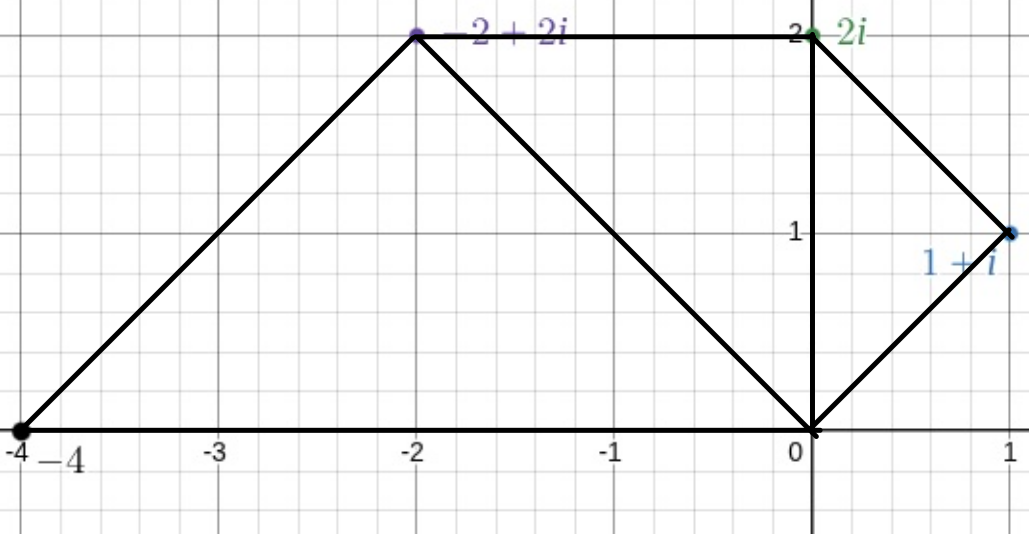
\includegraphics[scale=0.25]{./images/task33b.png}\\
This is for the sequence of $(1+i)^n$\\
This picture seems to be neatly expanding, the angle between the triangles are 45 degrees apart.\\

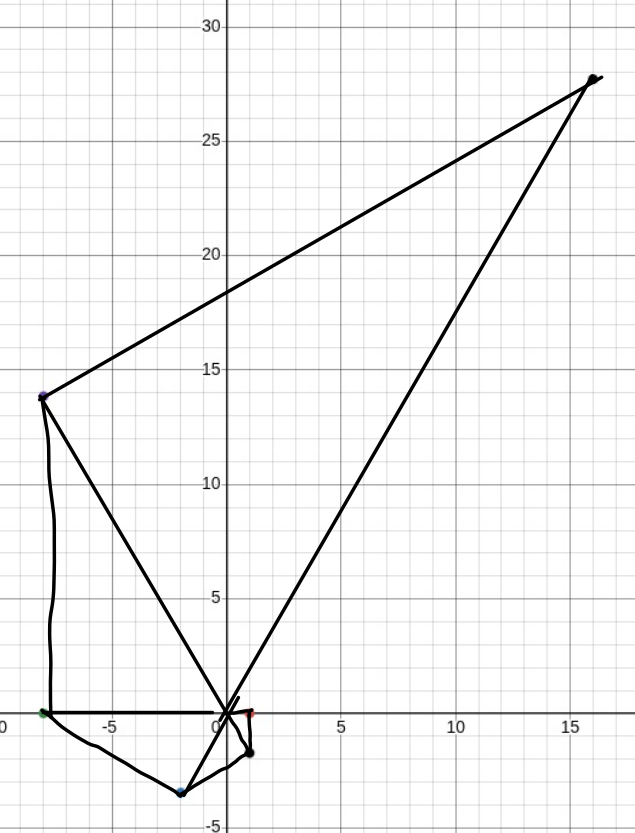
\includegraphics[scale=0.25]{./images/task33a.png}\\
This is for the sequence of $(1-\sqrt{3}i)^n$\\
Here, the picture seems to spiral out, and within task 15, this made sense because the numbers seemed to explode outwards.\\

\noindent{\bf Task 34} Describe what geometric shape is defined by each of these equations.\\
$z = x + yi$\\


\noindent{\bf a} $|z| = 1$\\
This is a unit circle, we can describe this as the magintude equal 1 at any given $x$ and $y$, which would make a circle.\\

\noindent{\bf b} $|z - 1| = 2$\\
This is a circle with the radius 2 and shifted 1 to the right, or centered on $(1,0)$.\\

\noindent{\bf c} $|z + 4i| = 3$\\
This is a circle with a radius of 3 shifted down 4. Centered on $(0,-4)$.\\

\noindent{\bf d} $|z| = |z - 1|$\\
This a line on $x = 0.5$.\\

\noindent{\bf e} $|z - i| = |z + i|$\\
This is a line on $y = 0$.\\

\noindent{\bf f} $|z - 2| =$ Re$z$ \\
This is a sideways opening parabola, opened to the right, where the vertex is $(1,0)$.\\

\noindent{\bf Task 35} Show that if $z$ is a nonzero complex number, then $z$/$|z|$ has modulus 1. Describe geometrically how $z$/$|z|$ relates to $z$.\\
$z = x + yi$\\
$|z| = \sqrt{x^2 + y^2}$\\

Before solving the question algebraically, we can discuss what this equation means.\\
If we think about $z$ being a vector of sorts, then $z/|z|$ would be the taking the vector and dividing off the length of the vector. 
Since both vectors have the same length, they are 1 length relative to each other.\\
So geometrically this would mean taking your complex number and scaling it to the length of itself.\\

$|\frac{z}{|z|}| = \frac{x+yi}{\sqrt{x^2 + y^2}}$\\
$|\frac{z}{|z|}| = x|z|^{-1} + yi|z|^{-1}$\\
$|\frac{z}{|z|}| = \sqrt{x^2|z|^{-2} + y^2|z|^{-2}}$\\
$|\frac{z}{|z|}| = \sqrt{\frac{x^2}{x^2 + y^2} + \frac{y^2}{x^2 + y^2}}$\\
$|\frac{z}{|z|}| = \sqrt{\frac{x^2 + y^2}{x^2 + y^2}}$\\
$|\frac{z}{|z|}| = \sqrt{1} = 1$\\



\noindent{\bf Task 36} Show that, if $\theta$ is any real number, then $\cos\theta + i\sin\theta$ has modulus 1.\\

Since, $\cos$ and $\sin$ both correlate to the unit circle, what ever the theta value is, together cosine and sine will add up to be the radius of the circle.\\


$|\cos\theta + i\sin\theta| = (\cos\theta + i\sin\theta)(\cos\theta - i\sin\theta)$\\
$|\cos\theta + i\sin\theta| = (\cos\theta)^2 + (\sin\theta)^2$\\
$|\cos\theta + i\sin\theta| = 1$\\


\noindent{\bf Task 37} Find the principal argument and one other argument for each number in task 26.\\

\noindent{\bf a} $z = i$\\
Since this is a simple rotation on the imaginary axis, Arg $z = \frac{\pi}{2}$.\\ 
Another Arg $z$ is $\frac{5\pi}{2}$.\\

\noindent{\bf b} $z = 1 + i$\\
Breaking this up into a triangle, it is easy to see that the triangle will have a base of 1 and height of i. 
If we then scale the triangle to the unit circle, we can see that this new triangle has $\frac{1}{\sqrt{2}}$ and $\frac{i}{\sqrt{2}}$.
Or, we could see that the hypotenuse is $\sqrt{2}$, which only happens on a 45 degree or $\frac{\pi}{4}$ triangle.\\

So, Arg $z = \frac{\pi}{4}$ and $\frac{9\pi}{4}$.\\

\noindent{\bf c} $z = -3$\\
Since this is a simple rotation on the real axis, Arg $z = \pi$.\\
Another Arg $z$ is $3\pi$.\\

\noindent{\bf d} $z = 3 - i\sqrt{3}$\\
Taking the modulus on this to find the hypotenuse, shows that this triangle is 30 60 90 triangle.\\
This is information, Arg $z = \frac{\pi}{6}$ and $\frac{13\pi}{6}$.\\


\noindent{\bf e} $z = -5 + 12i$\\
Taking the modulus shows that there is no easy pattern here, the given triangle is a pythagorean triple.
However, we are given the lengths of the sides, so we can use sine or cosine for the angle. 
I chose sine and did $\sin^{-1}{-5/13} + pi$, which equals $-0.384615384615$.
Adding two $\pi$ would result in $5.89856992256$


\noindent{\bf Task 38} Write each of the numbers from task 26 in polar form.\\
Using the last task, we have the $\theta$ for each set of numbers.\\


\noindent{\bf a} $z = i$\\
$1(\cos(\pi) + i\sin(\pi))$\\


\noindent{\bf b} $z = 1 + i$\\
$\sqrt{2}(\cos(\frac{\pi}{4}) + i\sin(\frac{\pi}{4}))$\\


\noindent{\bf c} $z = -3$\\
$3(\cos(\pi) + i\sin(\pi))$\\


\noindent{\bf d} $z = 3 - i\sqrt{3}$\\
$2\sqrt{3}(\cos(\frac{\pi}{6}) + i\sin(\frac{\pi}{6}))$\\


\noindent{\bf e} $z = -5 + 12i$\\
$13(\cos(-0.384615384615) + i\sin(-0.384615384615))$\\


\noindent{\bf Task 39} Find general formulas that conver between the rectangular form $x + yi$ and the polar $r(\cos\theta + i\sin\theta)$ of a complex number, and explain why they work.\\
For the formulas, $r = |z|$ was already given witihn the definition 1.4.2.\\

However, Arg $z$ was not provided a formula, but we can use sine and cosine to solve for the angle between the triangle. 
Since we can describe the real and imaginary parts as intructions for constructing the sides of a triangle, each side length corresponds with the real or imaginary part.
Using this knowledge we can find hypotenuse and complete the triangle. Then use either sine, cosine, or tangent to find the angle.\\

So, $\frac{\Re{z}}{|z|} = \cos\theta$\\
$\cos^{-1}{\frac{\Re{z}}{|z|}} = \theta$\\

Taking both cosine and sine would be very useful here because there will sometimes in which one angle will not describe both x and y.\\

\noindent{\bf Task 40} Use the angle sum formulas to show that for all $\alpha, \beta \in \mathbb{R}$, then\\
$(\cos\alpha + i\sin\alpha)(\cos\beta + i\sin\beta) = \cos(\alpha + \beta) + i\sin(\alpha + \beta)$.\\

Angle Sum Formulas:\\
$\cos(\alpha + \beta) = \cos\alpha\cos\beta - \sin\alpha\sin\beta$,\\
$\sin(\alpha + \beta) = \cos\alpha\sin\beta + \sin\alpha\cos\beta$.\\

This is pretty much given to the reader, by just looking at the formulas, we can see that the right side of the equation will convert to the first sum angle formulas.\\

$(\cos\alpha + i\sin\alpha)(\cos\beta + i\sin\beta) = \cos(\alpha + \beta) + i\sin(\alpha + \beta)$.\\
$\cos(\alpha)\cos(\beta) + i\cos(\alpha)\sin(\beta) + i\sin(\alpha)\cos(\beta) - \sin(\alpha)\sin(\beta) = \cos(\alpha + \beta) + i\sin(\alpha + \beta)$.\\
$\cos(\alpha)\cos(\beta) - \sin(\alpha)\sin(\beta) + i(\cos(\alpha)\sin(\beta) + \sin(\alpha)\cos(\beta)) = \cos(\alpha + \beta) + i\sin(\alpha + \beta)$.\\
Here this can be reduced using the formulas.\\
$\cos(\alpha + \beta) + i(\sin(\alpha + \beta)) = \cos(\alpha + \beta) + i\sin(\alpha + \beta)$.\\

Thus this statement is true.\\

\noindent{\bf Task 41}\\
The formula could be derived from finding both the $z$ and $w$ complex number polar forms and realising that the answer to the idea of similar triangles is that $zw$ must be equal to the polar form multiplication.\\ 

\noindent{\bf Task 42} Show that \textit{de Moivre's formula} is true: if $\theta \in \mathbb{R}$ and $n \in \mathbb{N}$, then\\
$(\cos\theta + i\sin\theta)^n = \cos n\theta + i\sin n\theta$.\\

Using task 39, we can see that doing the multiplication out, we would end up with a similiar set of circumstances. 
We could say that $\theta$ could be both $\alpha$ and $\beta$, and that we could just represent every power as a multiplication of two different angles.
Since we add both angles, this would lead to $n\theta$.\\

$(\cos\theta + i\sin\theta)(\cos\theta + i\sin\theta)(\cos\theta + i\sin\theta)^{n-2} = \cos(n\theta) + i\sin(n\theta)$\\
$(\cos(\theta)\cos(\theta) - \sin(\theta)\sin(\theta) + i(\cos(\theta)\sin(\theta) + \sin(\theta)\cos(\theta)))(\cos\theta + i\sin\theta)^{n-2} = $ \\
$\cos(n\theta) + i\sin(n\theta)$\\
$(\cos(2\theta) + i\sin(2\theta))(\cos\theta + i\sin\theta)^{n-2} = \cos(n\theta) + i\sin(n\theta)$\\

And the process can be repeated to $n$ amounts.\\



\noindent{\bf Task 43} Find $(1+i)^n$ and $(1-i\sqrt{3})$ for $n = 10,25,99$. Write your answers in the form $x + yi$.\\

$(1 + i)^{10} = 32(\cos(\frac{\pi}{2}) + i\sin(\frac{\pi}{2}))$\\
Here I simplified the fractional part of cosine and sine.\\
$(1+ i)^{10} = 32((0) + i(1))$\\


$(1 + i)^{25} = \sqrt{2}^{25}(\cos(\frac{\pi}{4}) + i\sin(\frac{\pi}{4}))$\\
$(1 + i)^{25} = \sqrt{2}^{25}(\sqrt{2}) + i(\sqrt{2}))$\\
$(1 + i)^{25} = \sqrt{2}^{24} + i\sqrt{2}^{24}$\\
$(1 + i)^{25} = 4096 + 4096i$\\


$(1 + i)^{99} = \sqrt{2}^{99}(\cos(\frac{3\pi}{4}) + i\sin(\frac{3\pi}{4}))$\\
$(1 + i)^{99} = \sqrt{2}^{99}((-\frac{1}{\sqrt{2}}) + i(\frac{1}{\sqrt{2}}))$\\
$(1 + i)^{99} = -\sqrt{2}^{98} + i\sqrt{2}^{98}$\\
$(1 + i)^{99} = -2^{49} + 2^{49}i$\\


$(1 - i\sqrt{3})^{10} = 2^{10}(\cos(\frac{2\pi}{3}) + i\sin(\frac{2\pi}{3}))$\\
$(1 - i\sqrt{3})^{10} = 2^{10}(-\frac{1}{2}) + i\frac{\sqrt{3}}{2})$\\
$(1 - i\sqrt{3})^{10} = -2^{9} + i2^{9}\sqrt{3})$\\

$(1 - i\sqrt{3})^{25} = 2^{25}(\cos(\frac{\pi}{3}) + i\sin(\frac{\pi}{3}))$\\
$(1 - i\sqrt{3})^{25} = 2^{25}(\cos(\frac{\pi}{3}) + i\sin(\frac{\pi}{3}))$\\
$(1 - i\sqrt{3})^{25} = 2^{25}(-(\frac{1}{2}) + i(\frac{\sqrt{3}}{2}))$\\
$(1 - i\sqrt{3})^{25} = -2^{24} + 2^{24}i\sqrt{3}$\\


$(1 - i\sqrt{3})^{99} = 2^{99}(\cos(\frac{99\pi}{3}) + i\sin(\frac{99\pi}{3}))$\\
$(1 - i\sqrt{3})^{99} = 2^{99}(\cos(33\pi) + i\sin(33\pi))$\\
$(1 - i\sqrt{3})^{99} = 2^{99}(-1)$\\
$(1 - i\sqrt{3})^{99} = -2^{99}$\\


\textbf{\large Chapter 2}


\noindent{\bf Task 44} What is the effect of each of these functions on point of the complex plane?\\


\noindent{\bf a} $z \mapsto z + i$\\
This Affine function is a translation up by 1 on the imaginary axis.\\


\noindent{\bf b} $z \mapsto iz$\\
The Affine function is a rotation by 1 on the imaginary axis.\\


\noindent{\bf c} $z \mapsto iz + 4$\\
This Affine function is a rotation by 1 on the imaginary axis and a translation of 4 on the real axis.\\


\noindent{\bf d} $z \mapsto (1 + i)z$\\
This is a rotation by 45 degrees and scale the complex number by $\sqrt{2}$.\\


\noindent{\bf e} $z \mapsto 3z + 6i$\\
This scales the vector up by 3, and translates it 6 in the imaginary axis.\\


\noindent{\bf f} $z \mapsto 3 + 4i - z$\\
This translates the vector by 3 in the real axis and 4 in the imaginary axis, while fliping the original complex number.\\


\noindent{\bf Task 45} Find an affine function that rotates your square by: $\pi/2$ and $\pi$.\\
I believe that $z \mapsto iz$ would rotate my sqaure by $\pi/2$ because the angle of $i$ is $\pi/2$.

I believe that $z \mapsto -1z$ would rotate my sqaure by $\pi$ because the angle of $-1$ is $pi$.\\


\noindent{\bf Task 46} Show that if $f(z) = az + b$ is an affine function, then $f$ has an inverse if and only if $a \neq 0$.\\ 

Since $a \neq 0$, then $f'(z) = \frac{z-b}{a}$ would be the inverse function of a given affine function. 
This must be the case because the operations of the affine function are reversed to find the original funciton.\\

\noindent{\bf Task 47}\\

\noindent{\bf a} $z \mapsto z + i$\\
$f^{-1}(z) = z - i$\\
The effects of this function will translate the complex number down one on the imaginary axis.\\


\noindent{\bf b} $z \mapsto iz$\\
$f^{-1}(z) = \frac{z}{i}$\\
$f^{-1}(z) = z(-i)$\\
The effects of this function will be, the complex number will be rotated by $\pi/2$ radians clockwise.\\


\noindent{\bf c} $z \mapsto iz + 4$\\
$f^{-1}(z) = (-i)(z - 4)$.\\
$f^{-1}(z) = -iz + 4i$.\\
The effects of this affine function will be that the complex number will be rotated $\pi/2$ radians clockwise and translated 4 up in along the imaginary axis.\\


\noindent{\bf d} $z \mapsto (1 + i)z$\\
$f^{-1}(z) = \frac{z}{1+i}$\\
$f^{-1}(z) = z(\frac{1}{2} - i\frac{1}{2})$\\
The effect of this affine function reverses the scaling done by the original function and rotates $\pi/2$ clockwise.\\

\noindent{\bf e} $z \mapsto 3z + 6i$\\
$f^{-1}(z) = \frac{z}{3} + 2i$\\
The effect of this affine function scales down the complex number and translates it up along the imaginary axis.\\

\noindent{\bf f} $z \mapsto 3 + 4i - z$\\
$f^{-1}(z) = -z - 3 - 4i$\\
The effect of this affine function reflects the complex number across the real axis, translates it down and to the left.\\



\noindent{\bf Task 48} What is the effect of these fucntions on points on the complex plane?\\

\noindent{\bf a} $z \mapsto \bar{z}$\\
This affine function would just reflect the complex number across the real axis.\\

\noindent{\bf b} $z \mapsto i\overline{z}$\\
This affine function would reflect then rotate $\pi/2$ radians counterclockwise.\\

\noindent{\bf c} $z \mapsto \bar{z} + 2i$\\
This affine function would reflect across the real axis and translate up 2 on the imaginary axis.\\

\noindent{\bf d} $z \mapsto -\bar{z} + 4$\\
The affine function would reflect on the the real axis, then traslated four to the right, or on the real axis.\\

\noindent{\bf e} $z \mapsto \bar{z} + 1$\\
The affine function would reflect across the real axis, then translate to the right, 1 on the real axis.\\


\noindent{\bf Task 49} Show that $f(z) = a\bar{z} + b$ has an inverse if and only if $a \neq 0$.\\
$f^{-1}(z) = z = a\bar{z} + b$\\
$f^{-1}(z) = z - b = a\bar{z}$\\
$f^{-1}(z) = \frac{z - b}{a} = \bar{z}$\\
Here, $a$ cannot be $0$.\\
$f^{-1}(z) = \overline{\frac{z - b}{a}} = z$\\

Thus, it is true that $f(z) = a\bar{z} + b$ has an inverse if and only if, $a \neq 0$.\\


\noindent{\bf Task 50}\\

\noindent{\bf a} $z \mapsto \bar{z}$\\
$f^{-1}(z) = \bar{z}$\\
This function is its own inverse.\\

The effect of this function is just reflecting the complex number across the real axis.\\


\noindent{\bf b} $z \mapsto i\overline{z}$\\
$f^{-1}(z) = \overline{\frac{z}{i}}$\\
$f^{-1}(z) = \overline{z(-i)}$\\

Since the function was a rotation of $\pi/2$ radians in the counter clock-wise direction, it would be the case that the inverse function would be a $\pi/2$ radians rotation clock-wise around the origin.\\ 


\noindent{\bf c} $z \mapsto \bar{z} + 2i$\\
$f^{-1}(z) = \overline{z - 2i}$\\

This functions effects are that the function will be translated 2 down along the imaginary axis, then the conjugate will be taken, which reflects the complex number across the real axis.\\

\noindent{\bf d} $z \mapsto -\bar{z} + 4$\\
$f^{-1}(z) = z - 4 = -\bar{z}$\\
$f^{-1}(z) = -z + 4 = \bar{z}$\\
$f^{-1}(z) = \overline{-z + 4} = z$\\

This function first reflects diagonally across the origin then translates the complex number 4 along the real axis.\\


\noindent{\bf e} $z \mapsto \bar{z} + 1$\\
$f^{-1}(z) = \overline{z - 1}$

This functino first translates the complex number by $-1$ along the real axis, then the conjugate gets taken, which reflects the complex number across the real axis.\\ 


Here, I applied the inverse of the conjugate, the conjugate, last as the final operation.\\ 


\noindent{\bf Task 51}\\
$z = a + bi$\\
$1/z = \frac{x-yi}{x^2+y^2}$\\

\noindent{\bf a} Show that $|1/z| = 1/|z|$. What does this equation mean geometrically?\\
$|1/z| = |\frac{x}{x^2+y^2} - i\frac{y}{x^2 + y^2}|$.\\
$|1/z| = \sqrt{\frac{x^2}{(x^2 + y^2)^2} + \frac{y^2}{(x^2+y^2)^2}}$.\\
$|1/z| = \sqrt{\frac{x^2+y^2}{(x^2+y^2)^2}}$.\\
$|1/z| = \sqrt{\frac{1}{x^2+y^2}}$.\\
$|1/z| = 1/\sqrt{x^2+y^2}$.\\

$1/|z| = 1/\sqrt{x^2 + y^2}$.\\

This equation would represent a scaler that is the magintude of the complex number.\\

\noindent{\bf b} Show that arg($1/z$) = -arg(z). What does this equation mean geometrically?\\

arg($1/z$)$ = \tan^{-1}(\frac{\frac{x}{x^2+y^2}}{\frac{-y}{x^2+y^2}})$\\
arg($1/z$)$ = \tan^{-1}(\frac{x}{-y})$\\
-arg(z) $ = -\tan^{-1}(\frac{x}{y})$\\

What this means geometrically is, the complex number did not change rotation, and instead rotated the other direction which aligns with the idea that when $i$ is in the denominator that the rotation will happen clockwise.\\


\noindent{\bf c} What is the effect of $z \mapsto 1/z$ on points of the unit circle $|z| = 1$?\\

The effect of this mapping is that the points on the unit circle now follow the direction clockwise instead of counter-clockwise.\\
This is basically reflecting the original point across the real axis.\\


\noindent{\bf d} What is the effect of $z \mapsto 1/z$ on points inside the unit circle (excluding 0)?\\

When $z$ is inside of the unit circle, the $1/z$ gets larger and larger the closer $z$ gets to zero.\\

\noindent{\bf e}What is the effect of $z \mapsto 1/z$ on points outside the unit circle?\\

Since in the last function the original value got closer to zero, in this function when $z$ gets farther away from the unit circle, the $1/z$ gets closer and closer to zero.\\


\noindent{\bf Task 52} The domain of $f: z \mapsto 1/z$ is $\mathbb{C} \ {0}$. Show that $f$ is one-to-one, and find $f^{-1}$.\\

Let's assume that we have two values, $a$ and $b$, and have $a = b$.\\
Then, $1/a = 1/b$, $\bar{a}/a = \bar{b}/b$, and $a = b$.\\
Thus, the function is one-to-one.\\

This proof uses the inverse which is: \\
$z = x + yi$.\\
$1/z = \frac{x-yi}{x^2+y^2}$.\\
$z = \frac{x^2+y^2}{x-yi} (\frac{x+yi}{x+yi})$.\\
$z = \frac{x^2+y^2}{x^2+y^2} (x+yi) $.\\
$z = x+yi$.\\

\noindent{\bf Task 53}\\


\noindent{\bf a} Show that arg($1/\bar{z}$) = arg z. What does this equation mean geometrically?\\
$z = x + yi, \bar{z} = x - yi$.\\
Using task 51, we can simplify very quickly,\\

arg($1/\bar{z}$) $= tan(\frac{x}{y})$\\
arg($1/\bar{z}$) $= tan(\frac{x}{y}) =$ arg($z$) \\

This explains geometrically that the imaginary and the real part of both positive when the reciprocal conjugate is taken. 
This would explain why they would have the same rotational angle.\\

\noindent{\bf b} Show that $z = 1/\bar{z}$ if and only if z is on the unit circle.\\

Using the defination for polar cordinates for complex numbers, we know that the magintude of the given complex number on the plane will have to be 1.\\
Then, $cos(\theta) + isin(\theta)$, and using the last section, we know that the angle of must also be the same.\\

Thus, only on the unit circle would it be possible for the $\bar{z}$ to be equal to the $z$.\\ 

\noindent{\bf c} Show that $z \mapsto 1/\bar{z}$ is its own inverse.\\

$1/\bar{z} = z$\\
$\bar{z} = 1/z$\\
$z = \overline{1/z}$\\

Just by doing the order of operations, we can see that the function is its own inverse.\\


\noindent{\bf d} Describe the function $z \mapsto 1/\bar{z}$ as a transformation of \mathbb{C}$\ {0} $\\

With the polar form, the $r$ will equal $\sqrt{\frac{x^2+y^2}{(x^2+y^2)^2}}$ and the given angles will be $\tan(\frac{x}{y})$.\\
So, it must be the case that every point will be scaled by that $r$, while the angle will stay the same.\\


\noindent{\bf Task 54}\\

\noindent{\bf a} Express the real and imaginary parts of $z^2$ in terms of the real and imaginary parts of z.\\


\noindent{\bf b} What is the effect of $z \mapsto z^2$ on vertical lines, of the form Re $z$ = constant?\\


\noindent{\bf c} What is the effect of $z \mapsto z^2$ on horizontal lines, of the form Im $z$ = constant?\\


\noindent{\bf Task 55}\\


\noindent{\bf a} Express the modulus and argument of $z^2$ in terms of the modulus and argument of $z$.\\


\noindent{\bf b} What is the effect of $z \mapsto z^2$ on circles centered at the origin?\\


\noindent{\bf c} What is the effect of $z \mapsto z^2$ on lines through the origin?\\


\noindent{\bf Task 56} Using your work from the previous two task, give as complete a description as you can of the function $z \mapsto z^2$ as a transformation.\\


\noindent{\bf Task 57}Let $R_+$ \textit{right half-plane}\\
$R_+ = {z: $ Re $z > 0}.$\\





\noindent{\bf Task 58}\\


\noindent{\bf Task 59}\\


\noindent{\bf Task 60}\\






\end{document}
